\documentclass[a4paper,12pt]{article}

%% Language and font encodings
\usepackage[T1]{fontenc}
\usepackage[polish]{babel}
\usepackage[utf8]{inputenc}
\usepackage{lmodern}
\selectlanguage{polish}

%% Sets page size and margins
%\usepackage[a4paper,top=2cm,bottom=2cm,left=2cm,right=4cm,asymmetric]{geometry}
\usepackage{geometry}


%% Useful packages
\usepackage[fleqn]{amsmath}%[fleqn]
\usepackage{xfrac} %\sfrac{}{}

\usepackage{titlesec}%titles
\titlelabel{\thetitle.\quad}
\let\savenumberline\numberline
\def\numberline#1{\savenumberline{#1.}}
\usepackage{etoolbox}%dots in TOC
\makeatletter
\patchcmd{\l@section}
{\hfil}
{\leaders\hbox{\normalfont$\m@th\mkern \@dotsep mu\hbox{.}\mkern \@dotsep mu$}\hfill}
{}{}
\makeatother

\usepackage{caption,graphicx}
\usepackage{float}
\usepackage{sidecap}
\usepackage[colorinlistoftodos]{todonotes}
\usepackage[colorlinks=true, allcolors=blue]{hyperref}

\usepackage{tikz}
\usepackage{tikz-qtree}
\usetikzlibrary{trees}
\usetikzlibrary{arrows,positioning,shapes,fit,calc,decorations.pathreplacing}
\usetikzlibrary{graphs}
\usetikzlibrary{graphs.standard}
\usepackage{forest}
\usepackage{tikzscale}
\usepackage{pgfgantt} %Diagramy gantta http://bay.uchicago.edu/CTAN/graphics/pgf/contrib/pgfgantt/pgfgantt.pdf
\usepackage{pgf}
\usepackage{caption}

\usepackage{fancybox}
\usepackage{listings}

\usepackage[colorinlistoftodos]{todonotes} %http://mirror.unl.edu/ctan/macros/latex/contrib/todonotes/todonotes.pdf

\usepackage{array,longtable}

\newcommand\floor[1]{\lfloor#1\rfloor} %PODŁOGA -> \floor
\newcommand\ceil[1]{\lceil#1\rceil} %SUFIT -> \ceil

\usepackage{fancyhdr}
\pagestyle{fancy}
\rhead{\thepage}
\lhead{\leftmark}
\rfoot{\thepage}
\lfoot{\rightmark}

%http://tex.stackexchange.com/questions/64170/which-package-to-use-for-writing-algorithms
\usepackage{algorithm}% http://ctan.org/pkg/algorithms
\usepackage{algpseudocode}% http://ctan.org/pkg/algorithmicx
\newcommand{\var}[1]{{\ttfamily#1}}% variable

\algnewcommand\algorithmicforeach{\textbf{for each}} %Algorithm foreach
\algdef{S}[FOR]{ForEach}[1]{\algorithmicforeach\ #1\ \algorithmicdo}

\usepackage{amsthm}
\usepackage[inline]{enumitem} %enumerations
\usepackage{multicol}

\theoremstyle{definition}%~ %%% <-  Note that space!
\newtheorem{lemma}{Lemat} %\begin{lemma} ... \end{lemma} LEMAT(?)
\newtheorem{remark}{Wniosek}%\begin{remark} ... \end{remark} WNIOSEK 
%\newtheorem*{remark*}{Wniosek}%\begin{remark} ... \end{remark} WNIOSEK bez liczby
\newtheorem{theorem}{Twierdzenie}%\begin{theorem} ... \end{theorem}
\newtheorem{fact}{Fakt} %\begin{fact} ... \end{fact}
\newtheorem*{fact*}{Fakt} %\begin{fact*} ... \end{fact*} Fakt
\newtheorem*{observation*}{Obserwacja}

\newtheorem{example}{Przykład}
\newtheorem*{example*}{Przykład} %\begin{example} ... \end{example}
\theoremstyle{definition}
\newtheorem{definition}{Definicja}%\begin{definition}{} ... \end{definition}
%\newtheorem*{definition*}{Definicja}
%\newtheorem*{hipoterm*}{Hipoteza}%\begin{hipoterm*}[] ... \end{hipoterm*}
\newtheorem{hipoterm}{Hipoteza}%\begin{hipoterm*}[] ... \end{hipoterm*}
\theoremstyle{problem}
\newtheorem{problem}{Problem}%\begin{problem}{} ... \end{problem}
\newtheorem*{problem*}{Problem}

\let\originalforall=\forall%FORALL
\renewcommand{\forall}{\mathop{\vcenter{\hbox{\Large$\originalforall$}}}}
\let\originalexists=\exists%EXISTS
\renewcommand{\exists}{\mathop{\vcenter{\hbox{\Large$\originalexists$}}}}

\usepackage{cancel} %skreślenie równania \xcancel{...} \cancel{} lub \bcancel{}

\usepackage{amsfonts}

\usepackage{comment}

\usepackage{xcolor,colortbl}
\usepackage{multirow}

%\usepackage{wrapfig} %wrap text around figure

\usepackage{pdfpages}%\includepdf{file}

\usepackage{etoolbox}
\let\bbordermatrix\bordermatrix
\patchcmd{\bbordermatrix}{8.75}{4.75}{}{}
\patchcmd{\bbordermatrix}{\left(}{\left[}{}{}
\patchcmd{\bbordermatrix}{\right)}{\right]}{}{}
%\bbordermatrix{}

\allowdisplaybreaks

\title{Struktury Dyskretne - Notatki}
\author{Piotr Parysek\\
\href{mailto:piotr.parysek@outlook.com}{piotr.parysek@outlook.com} }
\date{\today}

\begin{document}
\maketitle

\tableofcontents
\section{Ćwiczenia 6: 30-III-2017}
\subsection{Zadania}
\paragraph{Zad.1} Znajdź największy przepływ i najmniejsze cięcie w poniższej sieci. Uzasadnij poprawność rozwiązania. Cięcie proszę wskazać za pomocą odpowiedniego podziału zbioru wierzchołków.
\begin{figure}[H]
\centering
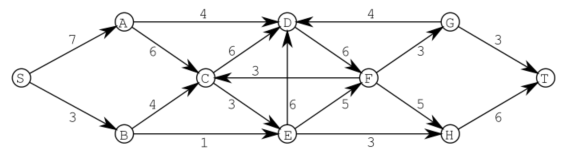
\includegraphics[width=.8\textwidth]{img/6_Z1}
\end{figure}

\paragraph{Zad.2} Oszacuj najlepiej jak potrafisz (z góry i z dołu) pojemność najmniejszego cięcia i wartość największego przepływu w podanej sieci.
\begin{figure}[H]
\centering
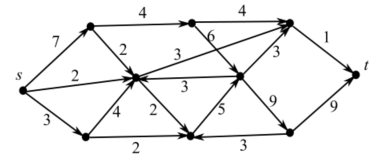
\includegraphics[width=.8\textwidth]{img/6_Z2}
\end{figure}

\paragraph{Zad.3} Rozważmy pewną sieć.
\begin{enumerate}[label=\alph*)]
\item Załóżmy, że wartość największego przepływu wynosi 10. Czy istnieje w rozważanej sieci cięcie o pojemności 8?
\item Załóżmy, że pojemność najmniejszego cięcia w sieci wynosi 10. Czy każdy przepływ w tej sieci ma wartość mniejszą niż 12?
\end{enumerate}


\paragraph{Zad.4} Załóżmy, że chcemy znaleźć największy przepływ w podanej nietypowej sieci $D_1$ z wieloma źródłami i ujściami. Przetłumacz problem na równoważny mu problem znalezienia odpowiedniego przepływu w standardowej sieci z jednym ujściem i jednym źródłem.
\begin{figure}[H]
\centering
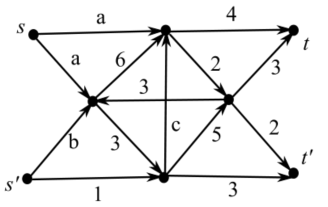
\includegraphics[width=.8\textwidth]{img/6_Z4}
\end{figure}

\paragraph{Zad.5} Chcemy rozstrzygnąć, czy w podanej nietypowej sieci istnieje dopuszczalny przepływ, w którym są spełnione zapotrzebowania wierzchołków. Liczby w wierzchołkach oznaczają zapotrzebowania: ujemne oznaczają, że wierzchołek chce o tyle więcej ,,dać” a dodatnie, że chce o tyle więcej ,,dostać”. Liczby na krawędziach oznaczają, jak zwykle, pojemność krawędzi. Przetłumacz problem na równoważny mu problem znalezienia odpowiedniego przepływu w standardowej sieci z jednym ujściem i jednym źródłem, w której zapotrzebowanie wszystkich wierzchołków (poza ujściem i źródłem) wynosi 0.
\begin{figure}[H]
\centering
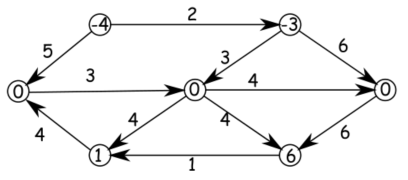
\includegraphics[width=.8\textwidth]{img/6_Z5}
\end{figure}

\paragraph{Zad.6} A to jeszcze bardziej nietypowa sieć. pojemność jednej krawędzi jest ograniczona z dołu i z góry podanymi liczbami. Podobnie jak w poprzednim zadaniu, Przetłumacz problem znalezienia dopuszczalnego przepływu w tej dziwnej sieci na równoważny mu problem znalezienia odpowiedniego przepływu w standardowej sieci.
\begin{figure}[H]
\centering
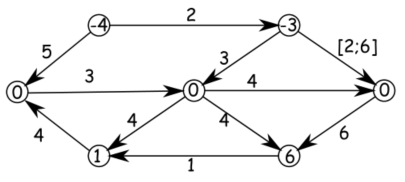
\includegraphics[width=.8\textwidth]{img/6_Z6}
\end{figure}

\subsection{Zadania Domowe B}
\paragraph{B1} Znajdź największy przepływ w poniższej sieci. Uzasadnij poprawność rozwiązania, wskazując odpowiednie Cięcie.
Jeśli rozwiązanie sprawia Państwu problemy, proszę  wykorzystać pomysł ścieżek rozszerzających z wykładu.
Na końcu proszę porównać rozwiązanie z rozwiązaniem otrzymanym przez zastosowanie gotowego narzędzia wykorzystującego algorytm Forda-Fulkersona, np. \url{https://visualgo.net/maxflow}

\paragraph{B2}
\begin{enumerate}[label=\alph*)]
\item Załóżmy, że w sieci, w której każda krawędź z ma pojemność 2, istnieje przepływ o wartości 13. Czy w tej sieci może istnieć Cięcie wyznaczone przez sześć strzałek?
\item Załóżmy, że w sieci, w której każda krawędź z ma pojemność 3, istnieje cięcie o pojemności 15, ale nie jest to Cięcie najmniejsze. Co można powiedzieć o wartości największego przepływu w tej sieci?
\item Dana jest sieć D, w której ze źródła wychodzą dokładnie cztery strzałki o pojemnościach równych 1,1,1 i 4. Do ujścia dochodzą również cztery strzałki, każda o pojemności równej 2. Ponadto wiadomo, że najmniejsze Cięcie w D jest wyznaczone przez 4 strzałki: pewne dwie spośród strzałek wychodzących ze źródła razem z dwiema spośród strzałek dochodzących do ujścia.
Co można powiedzieć o wartości największego przepływu w tej sieci?
\end{enumerate}

\paragraph{B3}
\begin{enumerate}[label=\alph*)]
\item Dana jest sieć $D$, w której każda krawędź z ma pojemność jeden. Uzasadnij, że w $D$ istnieje taki przepływ o największej wartości, że wartość przepływu na każdej z krawędzi wynosi jeden lub zero.

\textbf{Odpowiedź: }Zgodnie z twierdzeniem podanym na wykładzie, jeśli wartości na krawędziach ma wartości całkowite, to maksymalny przepływ w tej sieci również ma wartość całkowitą.
\item Narysuj przykład sieci, w której każda krawędź z ma pojemność jeden, ale istnieje największy przepływ, który na niektórych krawędziach ma wartości niecałkowite.

\textbf{Odpowiedź: }
\begin{figure}[H]
\centering
\begin{tikzpicture}[shorten >=1pt, auto, node distance=3cm, ultra thick,main node/.style={circle,draw,minimum size=.4cm,inner sep=0pt]}]%fill=black,
\begin{scope}[every node/.style={font=\sffamily\Large\bfseries}]
\node[main node] (v1) at (0,0) {1};
\node[main node] (v2) at (2,0) {2};
\node[main node] (v3) at (4,2) {3};
\node[main node] (v4) at (4,-2) {4};
\node[main node] (v5) at (6,0) {5};

%\node[main node] (v) at (,) {};
\end{scope}
\begin{scope}[every edge/.style={draw=black,ultra thick}]
\draw[->]  (v1) edge node{$1[1]$} (v2);
\draw[->]  (v2) edge node{$1[0.5]$} (v3);
\draw[->]  (v2) edge [right] node{$1[0.5]$} (v4);
\draw[->]  (v3) edge node{$1[0.5]$} (v5);
\draw[->]  (v4) edge [right] node{$1[0.5]$} (v5);
%\draw[->]  (v) edge node{} (v);
\end{scope}
\end{tikzpicture}
\caption*{Przykład: $s=1,\ t=5$ z zaznaczonym przepływem, powyżej wartości wag}
\end{figure}
\end{enumerate}


\paragraph{B4} Załóżmy, że interesuje nas największy przepływ w podanej nietypowej sieci D 1 z dwoma ujściami.
\begin{enumerate}[label=\alph*)]
\item Zbuduj sieć $D_2$ tradycyjną, czyli z jednym źródłem i jednym ujściem, w której problem znalezienia największego przepływu jest równoważny problemowi największego przepływu w $D_1$.
\item Opisz, w jaki sposób na podstawie największego przepływu w $D_2$ zdefiniować w $D_1$ przepływ o wartości $\mathsf{maxflow}(D_2)$.
\item Opisz, w jaki sposób na podstawie największego przepływu w $D_1$ zdefiniować w $D_2$ przepływ o wartości $\mathsf{maxflow}(D_1)$.
\end{enumerate}
Uwaga: proszę tych problemów nie rozwiązywać, tzn. nie trzeba wskazywać największych przepływów.

\paragraph{B5} Chcemy rozstrzygnąć, czy w podanej nietypowej sieci z podanymi zapotrzebowaniami wierzchołków istnieje dopuszczalny przepływ. Przetłumacz problem na równoważny mu problem znalezienia odpowiedniego przepływu w standardowej sieci, czyli sieci z jednym ujściem i jednym źródłem, w której zapotrzebowanie wszystkich wierzchołków (poza ujściem i źródłem) wynosi 0.
Uwaga: proszę problemu nie rozwiązywać, tzn. nie szukać dopuszczalnego przepływu.

\paragraph{B6} Chcemy rozstrzygnąć, czy w podanej bardzo nietypowej sieci $D$ istnieje dopuszczalny przepływ, w którym wartość przepływu na każdej krawędzi jest ograniczona z dołu i z góry podanymi liczbami. Tu zapotrzebowania wierzchołków wynoszą zero. Przetłumacz problem na równoważny mu problem znalezienia odpowiedniego przepływu w standardowej sieci, czyli sieci z jednym ujściem i jednym źródłem, w której zapotrzebowanie wszystkich wierzchołków (poza ujściem i źródłem) wynosi 0, a ograniczenia na krawędziach są tylko górne. Jak na podstawie odpowiedniego przepływu w standardowej sieci uzyskać dopuszczalny przepływ dla $D$?\\
Uwaga: proszę problemu nie rozwiązywać, tzn. nie szukać dopuszczalnego przepływu.

\begin{minipage}{.5\textwidth}
\begin{figure}[H]
\centering
\begin{tikzpicture}[->,>=stealth', auto,thick,main node/.style={circle,thick,draw}]
\node[main node] (v5) at (0,0) {};
\node[main node] (v6) at (3,0) {};
\node[main node] (v1) at (-2,3) {};
\node[main node] (v4) at (0,6) {};
\node[main node] (v7) at (3,6) {};
\node[main node] (v3) at (5,3) {};
\node[main node] (v2) at (1.5,3) {};
\draw  (v1) edge node [above] {$[13;15]$} (v2);
\draw  (v2) edge node [above] {$[3;7]$} (v3);
\draw  (v2) edge node [left] {$[10;10]$} (v4);
\draw  (v2) edge node [left] {$[1;2]$} (v5);
\draw  (v2) edge node [left] {$[1;5]$} (v6);
\draw  (v4) edge node [above] {$[6;8]$} (v7);
\draw  (v4) edge node [left] {$[0;5]$} (v1);
\draw  (v7) edge node [left] {$[2;3]$} (v2);
\draw  (v7) edge node [left] {$[1;7]$} (v3);
\draw  (v3) edge node [left] {$[4;7]$} (v6);
\draw  (v6) edge node [below] {$[11;12]$}(v5);
\draw  (v5) edge node [left] {$[13;17]$} (v1);
\end{tikzpicture}
\caption*{(1)}
\end{figure}
\end{minipage}% 
\begin{minipage}{.5\textwidth}
\begin{figure}[H]
\centering
\begin{tikzpicture}[->,>=stealth', auto,thick,main node/.style={circle,thick,draw}]
\node[main node] (v5) at (0,0) {1};
\node[main node] (v6) at (3,0) {6};
\node[main node] (v1) at (-2,3) {0};
\node[main node] (v4) at (0,6) {-4};
\node[main node] (v7) at (3,6) {-3};
\node[main node] (v3) at (5,3) {4};
\node[main node] (v2) at (1.5,3) {0};
\draw  (v1) edge node [above] {$2$} (v2);
\draw  (v2) edge node [above] {$4$} (v3);
\draw  (v2) edge node [left] {$0$} (v4);
\draw  (v2) edge node [left] {$1$} (v5);
\draw  (v2) edge node [left] {$4$} (v6);
\draw  (v4) edge node [above] {$2$} (v7);
\draw  (v4) edge node [left] {$5$} (v1);
\draw  (v7) edge node [left] {$1$} (v2);
\draw  (v7) edge node [left] {$6$} (v3);
\draw  (v3) edge node [left] {$3$} (v6);
\draw  (v6) edge node [below] {$1$}(v5);
\draw  (v5) edge node [left] {$4$} (v1);
\end{tikzpicture}
\caption*{(2)}
\end{figure}
\end{minipage}\\% 
\begin{minipage}{.5\textwidth}
\begin{figure}[H]
\centering
\begin{tikzpicture}[->,>=stealth', auto,thick,main node/.style={circle,thick,draw}]
\node[main node] (v5) at (0,0) {1};
\node[main node] (v6) at (3,0) {6};
\node[main node] (v1) at (-2,3) {0};
\node[main node] (v4) at (0,6) {-4};
\node[main node] (v7) at (3,6) {-3};
\node[main node] (v3) at (5,3) {4};
\node[main node] (v2) at (1.5,3) {0};
\node[main node,color=blue] (vS) at (1.5,8) {S};
\node[main node,color=blue] (vT) at (4,-1.5) {T};
\draw  (v1) edge node [above] {$2$} (v2);
\draw  (v2) edge node [above] {$4$} (v3);
\draw  (v2) edge node [left] {$0$} (v4);
\draw  (v2) edge node [left] {$1$} (v5);
\draw  (v2) edge node [left] {$4$} (v6);
\draw  (v4) edge node [above] {$2$} (v7);
\draw  (v4) edge node [left] {$5$} (v1);
\draw  (v7) edge node [left] {$1$} (v2);
\draw  (v7) edge node [left] {$6$} (v3);
\draw  (v3) edge node [left] {$3$} (v6);
\draw  (v6) edge node [below] {$1$}(v5);
\draw  (v5) edge node [left] {$4$} (v1);
\draw[color=blue]  (vS) edge node [left] {4} (v4);
\draw[color=blue]  (vS) edge node [left] {3} (v7);
\draw[color=blue]  (v5) edge node [left] {3} (vT);
\draw[color=blue]  (v6) edge node [left] {3} (vT);
\draw[color=blue]  (v3) edge node [left] {3} (vT);
\end{tikzpicture}
\caption*{(3)}
\end{figure}
\end{minipage}% 
\begin{minipage}{.5\textwidth}
Graf nie ma rozwiązania

W (1) istnieje rozwiązanie wtedy i tylko wtedy, gdy w sieci (3) istnieje przepływ nasycający wszystkie strzałki wychodzące ze źródła $S$ i wszystkie wchodzące do ujścia $T$
\end{minipage}
\end{document}
